\documentclass[10pt]{article}
\usepackage{mathtools}
\usepackage{amsmath}
\usepackage{tabularx}
\usepackage{graphicx}
\usepackage{flexisym}
\usepackage{listings}
\usepackage{xcolor}
\usepackage{hyperref}

\begin{document}
\setlength\parindent{1pt}
\title{Project 2}
\author{Andrei Kukharenka and Anna Gribkovskaya \\  
FYS 4150 
}

\maketitle
\begin{abstract}
In this work we solve the Schr\"{o}dinger's equation for electrons confined in a small area by applying the Jacobi method for the matrix diagonalization. 
\end{abstract}
\clearpage 


\section{Introduction}
\newpage
\section{Problem Formulation}
In this project we consider have solved Schr\"{o}dinger's equation for electrons confined in a small area. First we took a one electron case and after this moved to a two-electrons repelling due to Coloubm interaction. 


We are first interested in the solution of the radial part of Schr\"{o}dinger's equation for one electron. 

\begin{equation*}
  -\frac{\hbar^2}{2 m} \left ( \frac{1}{r^2} \frac{d}{dr} r^2
  \frac{d}{dr} - \frac{l (l + 1)}{r^2} \right )R(r) 
     + V(r) R(r) = E R(r).
\end{equation*}
The potential $V(r)$  in the equation is a harmonic oscillator potential $(1/2)kr^2$ and $E$ is the energy of the harmonic oscillator. 

The boundary conditions are $u(0)=0$ and $u(\infty)=0$.

Assuming spherical symmetry and considering the orbital momentum $l=0$ we made some simple transformations and variable substitutions. Now the equation reads as


\begin{equation}
-\frac{d^{2}}{d\rho ^{2}}u(\rho )+\rho ^{2}u(\rho )=\lambda u(\rho )
\end{equation}

Using the standard expression for $u^{\prime \prime }$we obtain 
\begin{equation}
u^{\prime \prime }=\frac{u(\rho +h)-2u(\rho )+u(\rho -h)}{h^{2}}+O(h^{2})
\end{equation}

where $h$ is our step, given by

\begin{equation}
h=\frac{\rho _{\mathrm{max}}-\rho _{\mathrm{min}}}{n_{\mathrm{step}}}
\end{equation}

where $\rho _{\mathrm{max}}$ and $\rho _{\mathrm{min}}$ are given by boundary conditions. We assume $\rho _{\mathrm{min}}=0$, and define $\rho_{\mathrm{max}}$ as a most suitable for the applied algorithm.

Value of $\rho $ is given by

\begin{equation}
\rho _{i}=\rho _{\mathrm{min}}+ih\hspace{1cm}i=0,1,2,\dots ,n_{\mathrm{step}}
\end{equation}
we can rewrite the Schr\"{o}dinger equation for $\rho _{i}$ as

\begin{equation}
-\frac{u_{i+1}-2u_{i}+u_{i-1}}{h^{2}}+V_{i}u_{i}=\lambda u_{i}
\end{equation}
where $V_{i}=\rho _{i}^{2}$ is the harmonic oscillator potential. 

The diagonal matrix element are defined as

\begin{equation}
d_{i}=\frac{2}{h^{2}}+V_{i}
\end{equation}
the non-diagonal matrix element are
defined as 

\begin{equation}
e_{i}=-\frac{1}{h^{2}}
\end{equation}

In this case the Schr\"{o}dinger equation takes the following form

\begin{equation}
d_{i}u_{i}+e_{i-1}u_{i-1}+e_{i+1}u_{i+1}=\lambda u_{i}
\end{equation}
where $u_{i}$ is unknown. We can write the last equation as a matrix $%
\mathbf{A}$ eigenvalue problem

\[
\left( 
\begin{array}{ccccccc}
d_{1} & e_{1} & 0 & 0 & \dots  & 0 & 0 \\ 
e_{1} & d_{2} & e_{2} & 0 & \dots  & 0 & 0 \\ 
0 & e_{2} & d_{3} & e_{3} & 0 & \dots  & 0 \\ 
\dots  & \dots  & \dots  & \dots  & \dots  & \dots  & \dots  \\ 
0 & \dots  & \dots  & \dots  & \dots  & d_{n_{\mathrm{step}}-2} & e_{n_{%
		\mathrm{step}}-1} \\ 
0 & \dots  & \dots  & \dots  & \dots  & e_{n_{\mathrm{step}}-1} & d_{n_{%
		\mathrm{step}}-1}%
\end{array}%
\right) \left( 
\begin{array}{c}
u_{1} \\ 
u_{2} \\ 
\dots  \\ 
\dots  \\ 
\dots  \\ 
u_{n_{\mathrm{step}}-1}%
\end{array}%
\right) =\lambda \left( 
\begin{array}{c}
u_{1} \\ 
u_{2} \\ 
\dots  \\ 
\dots  \\ 
\dots  \\ 
u_{n_{\mathrm{step}}-1}%
\end{array}%
\right) 
\]%
or if we wish to be more detailed, we can write the tridiagonal matrix $%
\mathbf{A}$ as

\[
\left( 
\begin{array}{ccccccc}
\frac{2}{h^{2}}+V_{1} & -\frac{1}{h^{2}} & 0 & 0 & \dots  & 0 & 0 \\ 
-\frac{1}{h^{2}} & \frac{2}{h^{2}}+V_{2} & -\frac{1}{h^{2}} & 0 & \dots  & 0
& 0 \\ 
0 & -\frac{1}{h^{2}} & \frac{2}{h^{2}}+V_{3} & -\frac{1}{h^{2}} & 0 & \dots 
& 0 \\ 
\dots  & \dots  & \dots  & \dots  & \dots  & \dots  & \dots  \\ 
0 & \dots  & \dots  & \dots  & \dots  & \frac{2}{h^{2}}+V_{n_{\mathrm{step}%
	}-2} & -\frac{1}{h^{2}} \\ 
0 & \dots  & \dots  & \dots  & \dots  & -\frac{1}{h^{2}} & \frac{2}{h^{2}}%
+V_{n_{\mathrm{step}}-1}%
\end{array}%
\right) 
\]
\section{Mathematical methods}
\newpage
\section{Results and discussion}

\begin{table}
  \caption{One electron Jacobi.}
  \label{tab:one}
  \begin{center}
    \begin{tabular}{c|c|c|c|c}
    \hline
		$N$ & $Number of rotations$ & $\lambda_1$ & $\lambda_2$ & $\lambda_3$ \\
        \hline
	$	50 $  & $ 4036  $ & $2.77921$ & $6.65469$ & $10.5485$ \\
	$	100$  & $ 16521 $ & $2.88836$ & $6.82895$ & $10.7813$ \\
	$	200$  & $ 66745 $ & $2.94388$ & $6.91491$ & $10.8925$ \\
	$	300$  & $ 150755$ & $2.96252$ & $6.94338$ & $10.9288$ \\
	$	400$  & $ 269516$ & $2.97186$ & $6.95757$ & $10.9468$ \\

	\end{tabular}
  \end{center}
\end{table}

\begin{table}
  \caption{Two electrons Jacobi. N=200}
  \label{tab:two}
	\begin{center}
    \begin{tabular}{c|c|c|c|c}
    \hline
		$\omega$ & $Number\ of\ rotations$ & $\lambda_1$ & $\lambda_2$ & $\lambda_3$ \\
        \hline
		$0.01$ & $59717$ & $0.105776$ & $0.141516$  & $0.178049$ \\ 
		$0.5$  & $64207$ & $2.25271 $ & $4.17817 $  & $6.13601$ \\ 
		$1  $  & $64662$ & $4.11774 $ & $8.01741 $  & $11.966$ \\
		$5  $  & $66625$ & $17.8299 $ & $37.6929 $  & $57.7022$ \\

	\end{tabular}
  \end{center}
\end{table}


\begin{figure}
  \begin{center}
    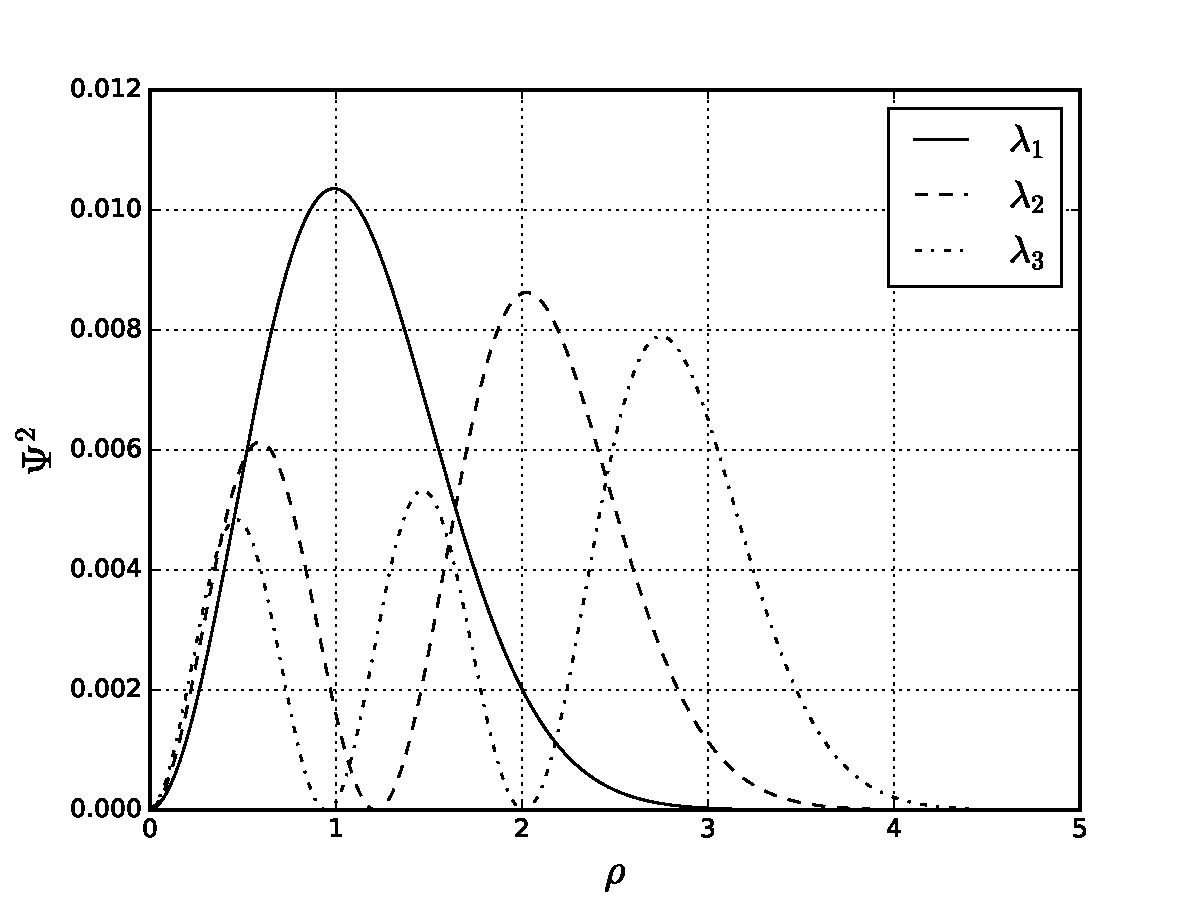
\includegraphics[scale=0.7]{one_electron}
    \caption{One electron}
    \label{fig:one_electron}
  \end{center}
\end{figure}

\begin{figure}
  \begin{center}
    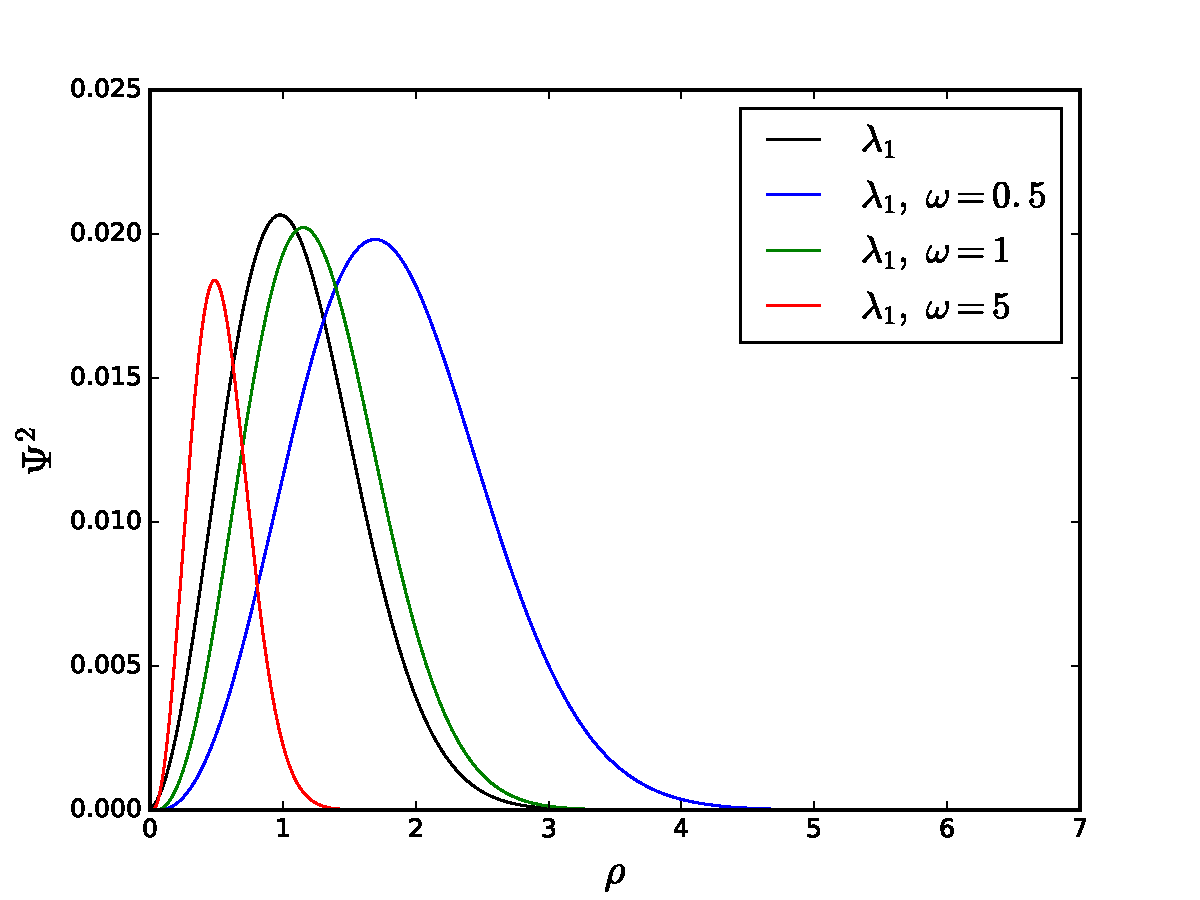
\includegraphics[scale=0.7]{compare}
    \caption{compare}
    \label{fig:compare}
  \end{center}
\end{figure}
\newpage
\begin{figure}
  \begin{center}
    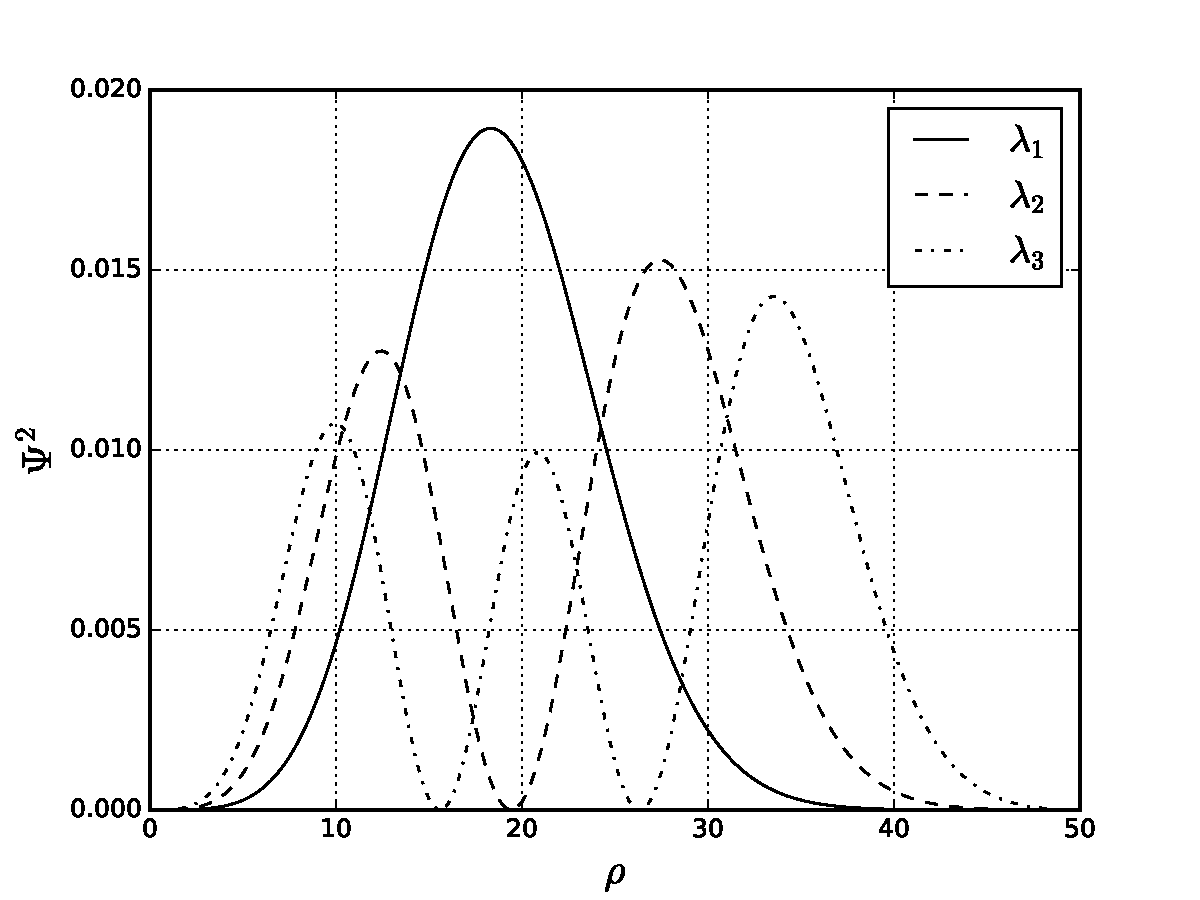
\includegraphics[scale=0.7]{two_001}
    \caption{0.01}
    \label{fig:omega_0.01}
  \end{center}
\end{figure}
\newpage

\begin{figure}
  \begin{center}
    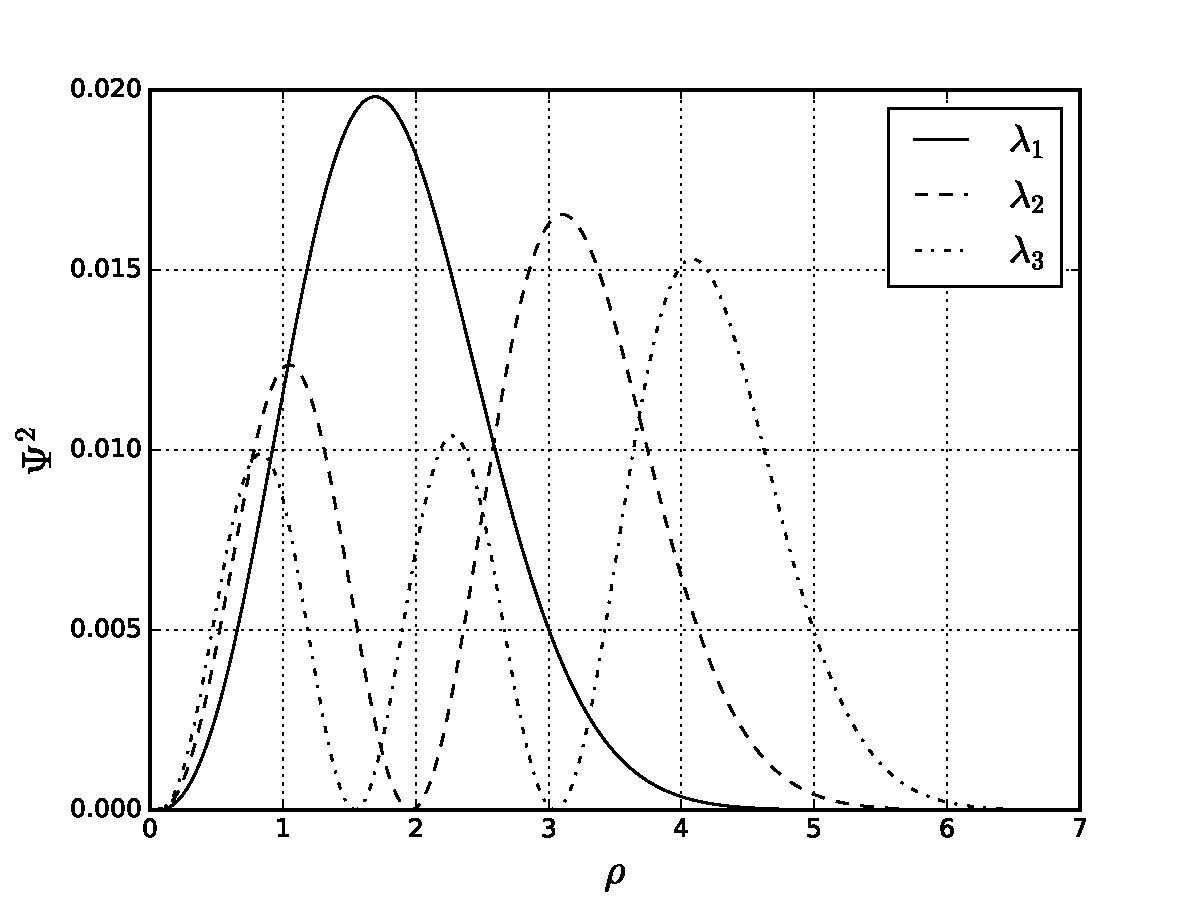
\includegraphics[scale=0.7]{two_05}
    \caption{0.5}
    \label{fig:omega_0.5}
  \end{center}
\end{figure}
\newpage

\begin{figure}
  \begin{center}
    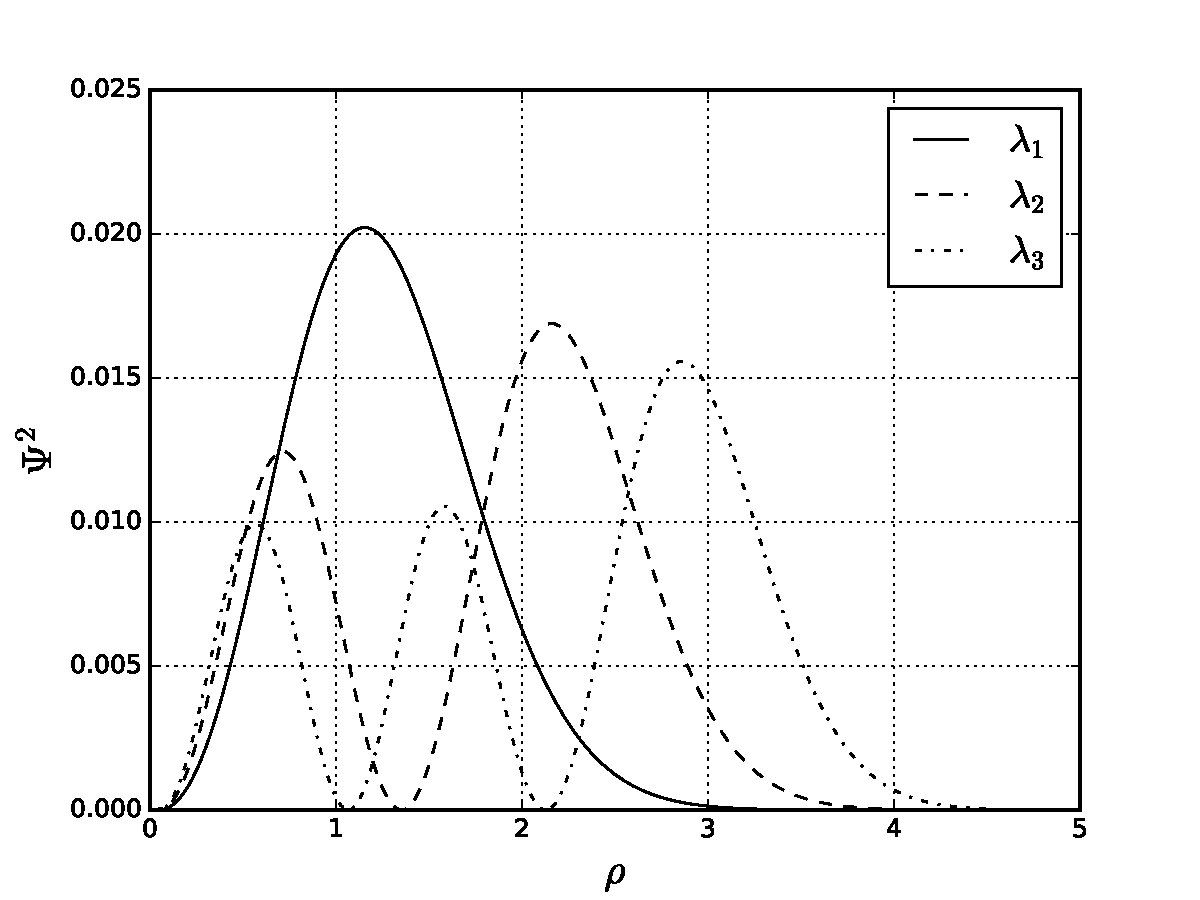
\includegraphics[scale=0.7]{two_1}
    \caption{1}
    \label{fig:omega_1}
  \end{center}
\end{figure}
\newpage

\begin{figure}
  \begin{center}
    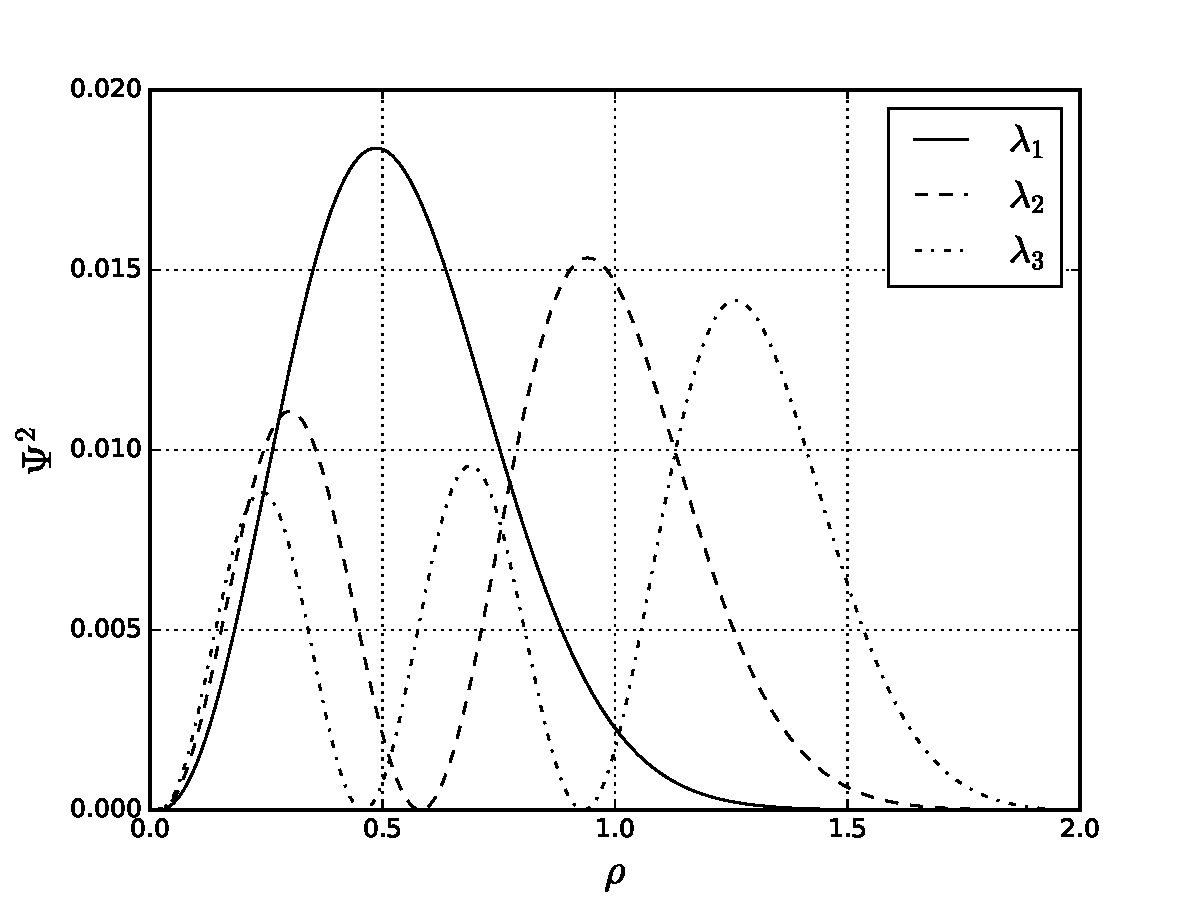
\includegraphics[scale=0.7]{two_5}
    \caption{5}
    \label{fig:omega_5}
  \end{center}
\end{figure}
\newpage


\section{Conclusion and further research}

\newpage
\begin{thebibliography}{2}
\bibitem{one} 
Morten Hjorth-Jensen. 
\textit{Computational Physics
}. 
Lecture Notes Fall 2015, August 2015.
 W. Press, B. Flannery, S. Teukolsky, W. Vetterling, Numerical Recipes in C++, The art of scientific Computing (Cambridge University Press, 1999)

\bibitem{two} 
W. Press, B. Flannery, S. Teukolsky, W. Vetterling 
\textit{Numerical Recipes in C++, The art of scientific Computing}. 
Cambridge University Press, 1999.
 
\end{thebibliography}

\end{document}
